\clearpage
\section{Auswertung}
\subsection{Pockels-Effekt}
Um den elektrooptischen Koeffizienten $r_{41}$ von ADP berechnen zu können, benutzten wir zwei verschiedene Methoden, um die Spannung $U_{\lambda/2}$, welche die Polarisation des einfallenden Lichtes um $90\,^{\circ}$ dreht.\\
\subsubsection{Sägezahnmethode}
Wir benutzten einen Spannungsgenerator, welcher ein Sägezahnsignal mit der Frequenz $\nu=30 Hz$ generiert. Die Spannung steigt daher konstant an. Dies bewirkt ein sinusförmiges Signal an der Fotodiode. \\
\begin{figure}[h]
\begin{center}
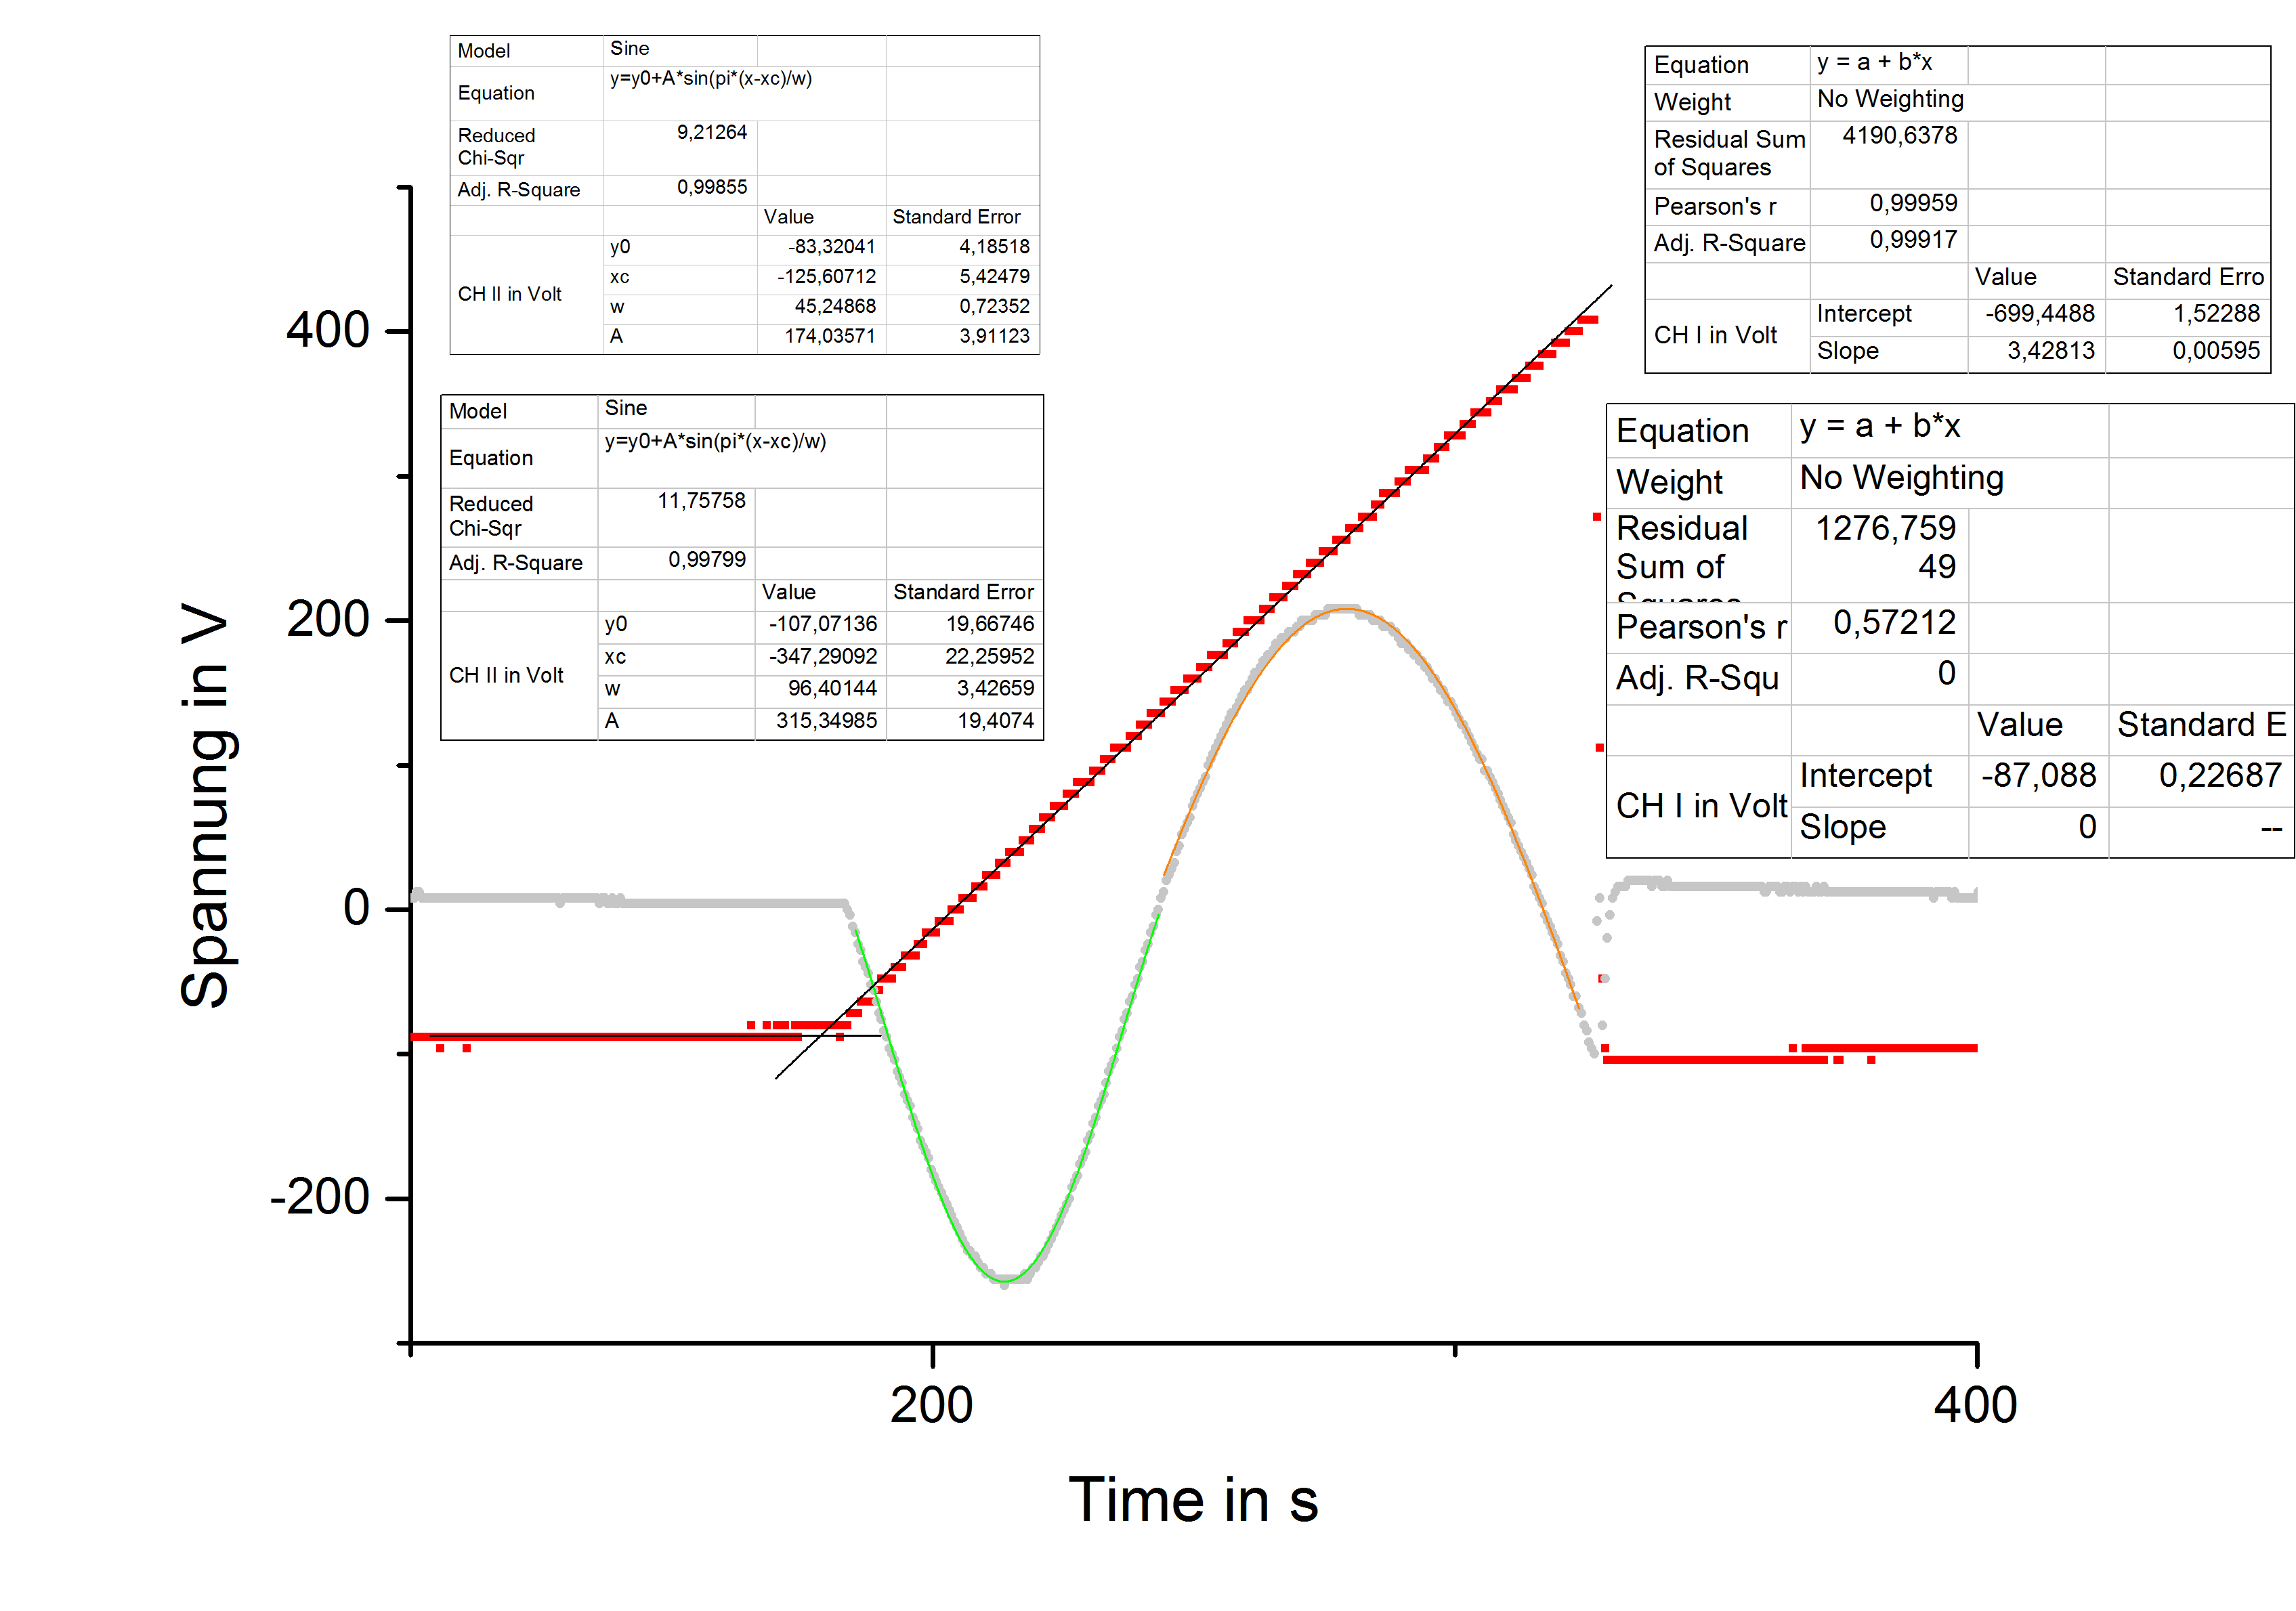
\includegraphics[scale=0.6]{anpassung1.png}
\caption{Durch Sägezahnspannung erzeugtes Signal}
\end{center}
\end{figure}
\clearpage
Wir entschlossen uns, an den negativen wie den positiven Peak des Signals der Fotodiode eine Sinuskurve zu fitten und mithilfe dieser die Zeiten zu bestimmen, zu welchen sie auftreten. Mithilfe der Differenz der zugehörigen Spannungen, welche zu den so bestimmten Zeiten bei dem Sägezahnsignal auftreten, lässt sich $U_{\lambda/2}$ bis auf einen Korrekturfaktor bestimmen. \\
Die Sinus-Fits haben die Form \[y=y_{0}+A*\sin(\pi*\frac{(x-x_{c})}{w})\]. Tiefpunkte erhält man dabei bei \[\frac{x-x_{c}}{w}=\frac{4k-1}{2}\], wobei $k\in \mathbb{Z}$ gilt. Analog gilt für Hochpunkte: \[\frac{x-x_{c}}{w}=\frac{4k-3}{2}\]. Für die Fehler folgt somit, wenn man nach x auflöst und die Gauss'sche Fehlerfortpflanzung verwendet: \[s_{x_{tief}}=\sqrt{(\frac{4k-1}{2})^{2}*(s_{w})^{2}+(s_{x_{c}})^{2}}\] und \[s_{x_{tief}}=\sqrt{(\frac{4k-3}{2})^{2}*(s_{w})^{2}+(s_{x_{c}})^{2}}\]. Der Fehler ist also am geringsten für $k_{tief}=0$ und $k_{hoch}=1$. Wie man bei der Betrachtung der Zeiten, zu welchen die Peaks etwa auftreten, jedoch sieht, gilt für unsere Fits $k_{tief}=4$ und $k_{hoch}=3$. Dies liegt am Auswerteprogramm Origin, welches wir verwendeten und welches die Fits auf diese Art erstellte. Um etwas kleinere Fehler zu erhalten, beschlossen wir, die Anfangszeit des Signals als Startpunkt festzusetzen. Aus diesem Grund berechneten wir den Schnittpunkt von linearem Fit der ansteigenden Sägezahnspannung und dem flachen, konstanten Bereich desselben Kanals zuvor (s. Diagramm). Somit erhielten wir für die Anfangszeit:\\
\[m*x+c=d\]
\[\Leftrightarrow x=\frac{d-c}{m}\]
\[\Rightarrow s_{x}=\sqrt{(\frac{s_{d}}{m})^{2}+(\frac{s_{c}}{m})^{2}+(\frac{(d-c)*s_{m}}{m^{2}})^{2}}\]
Den so erhaltenen Wert zogen wir mitsamt Fehler von den bisherigen Werten für die Zeit ab. Somit erhielten wir für das Diagramm:\\
\begin{figure}[h]
\begin{center}
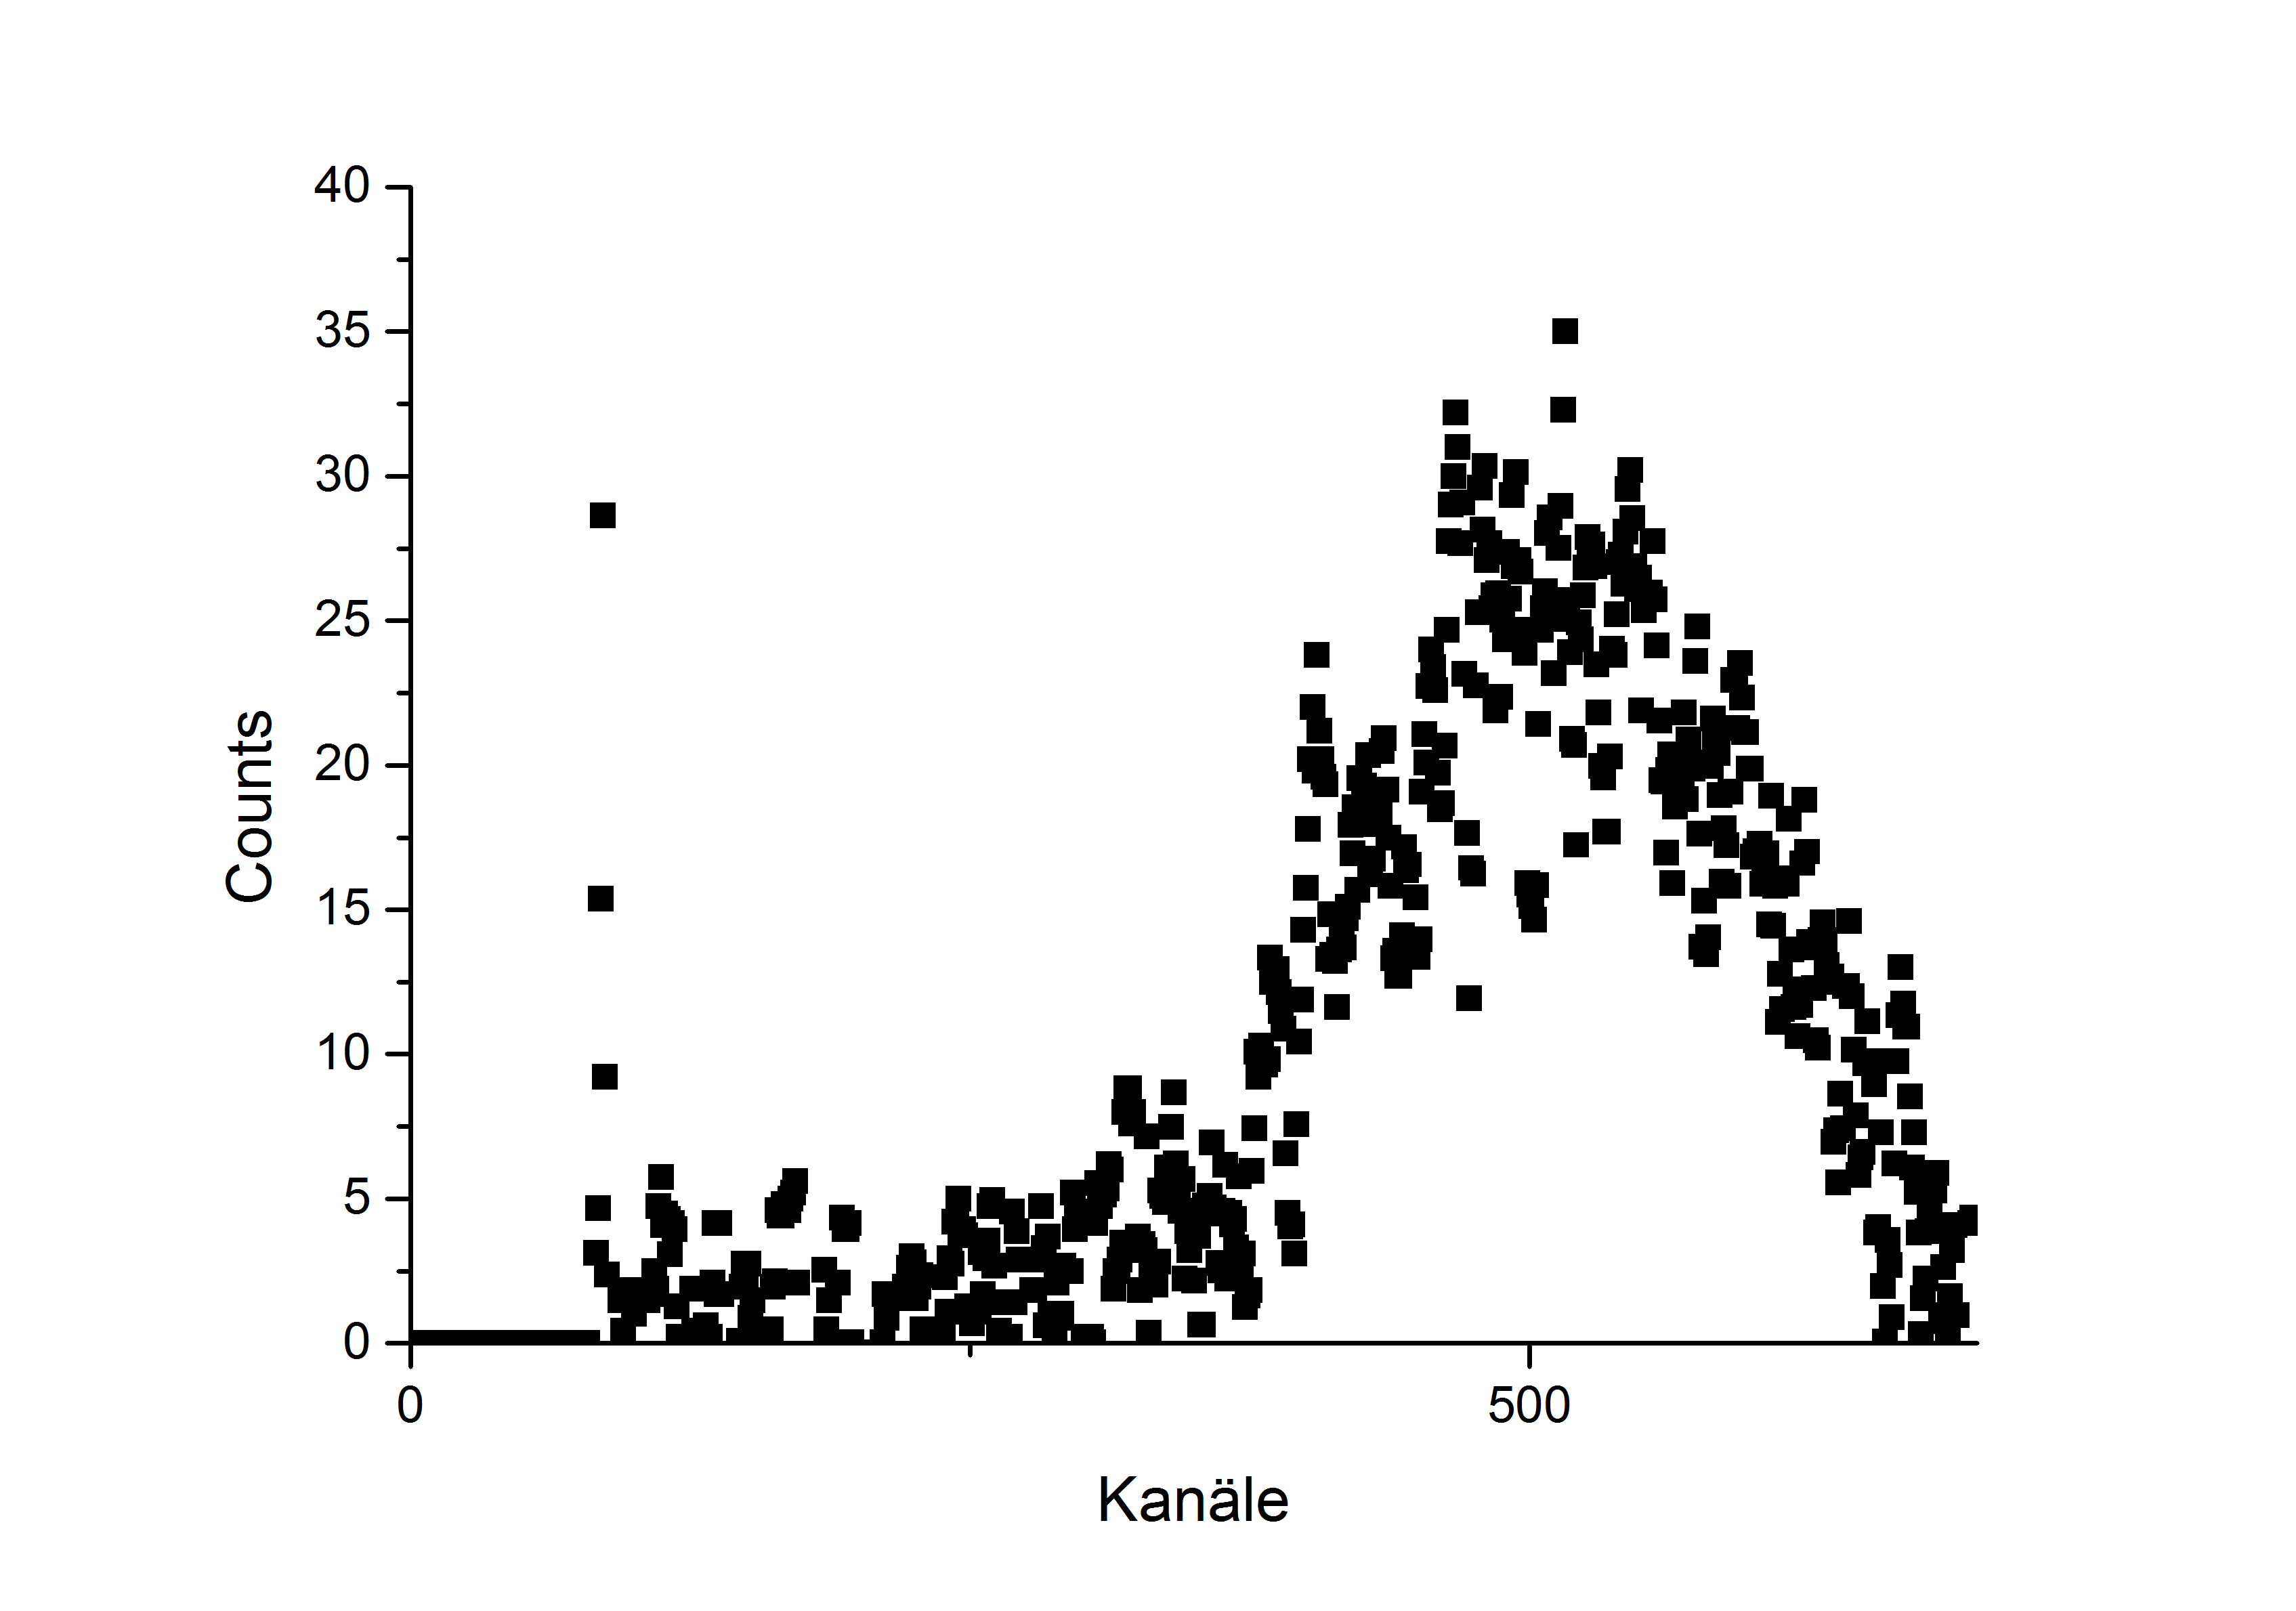
\includegraphics[scale=0.6]{korrigiert.png}
\caption{Durch Sägezahnspannung erzeugtes korrigiertes Signal}
\end{center}
\end{figure}
\clearpage
Damit erhielten wir $k_{tief}=1$ und $k_{hoch}=2$, was zwar zu einer Reduktion des Fehlers führt, jedoch noch immer nicht das bestmögliche Ergebnis darstellt. Wir entschlossen uns dennoch, mit diesem Ergebnis weiterzurechnen, weil wir den Nullpunkt nicht willkürlich verschieben wollten. Somit erhielten wir für die Zeiten, bei denen die Peaks liegen:\\
$x_{tief}=(35,2\pm1,4)s$\\
$x_{hoch}=(101\pm6)s$\\
Nun setzten wir diese Werte jeweils in die Geradengleichung $y=m*x+c$ (s. Diagramm), welche wir für die Sägezahnspannung erhielten, ein. Um die Fehler zu berechnen, verwendeten wir die Gauss'sche Fehlerfortpflanzung:\\
$s_{y}=\sqrt{m^{2}*s_{x}^{2}+s_{c}^{2}+x^{2}*s_{m}^{2}}$\\
Die Differenz der beiden so erhaltenen Spannungen ist:\\
$U=y_{hoch}-y_{tief}=224,2 V$\\
$\Rightarrow s_{U}=\sqrt{s_{y_{tief}}^{2}+s_{y_{hoch}}^{2}}=20,3 V$\\
Da die Fehler allgemein ziemlich groß waren, haben wir die Fehler des Oszilloskops vernachlässigt.\\
Die somit errechnete Spannung entspricht noch nicht zwangsläufig der Spannung $U_{\lambda/2}$, welche wir errechnen sollten. Dies ist der Fall, da das Computerprogramm von einer Dämpfung um den Faktor 100 bei der Sägezahnspannung rechnete und daher die für diese erhaltenen Werte mit demselben Faktor multiplizierte. Um den tatsächlichen Dämpfungsfaktor zu errechnen, verglichen wir am Oszilloskop an unterschiedlichen Kanälen das normale mit dem gedämpften Signal, um Rückschlüsse ziehen zu können. Wir benutzten erneut Sinus-Fits für die Peaks, wie in den folgenden Diagrammen zu sehen ist, welches eines der drei Messreihen darstellt:\\
\begin{figure}[h]
\begin{center}
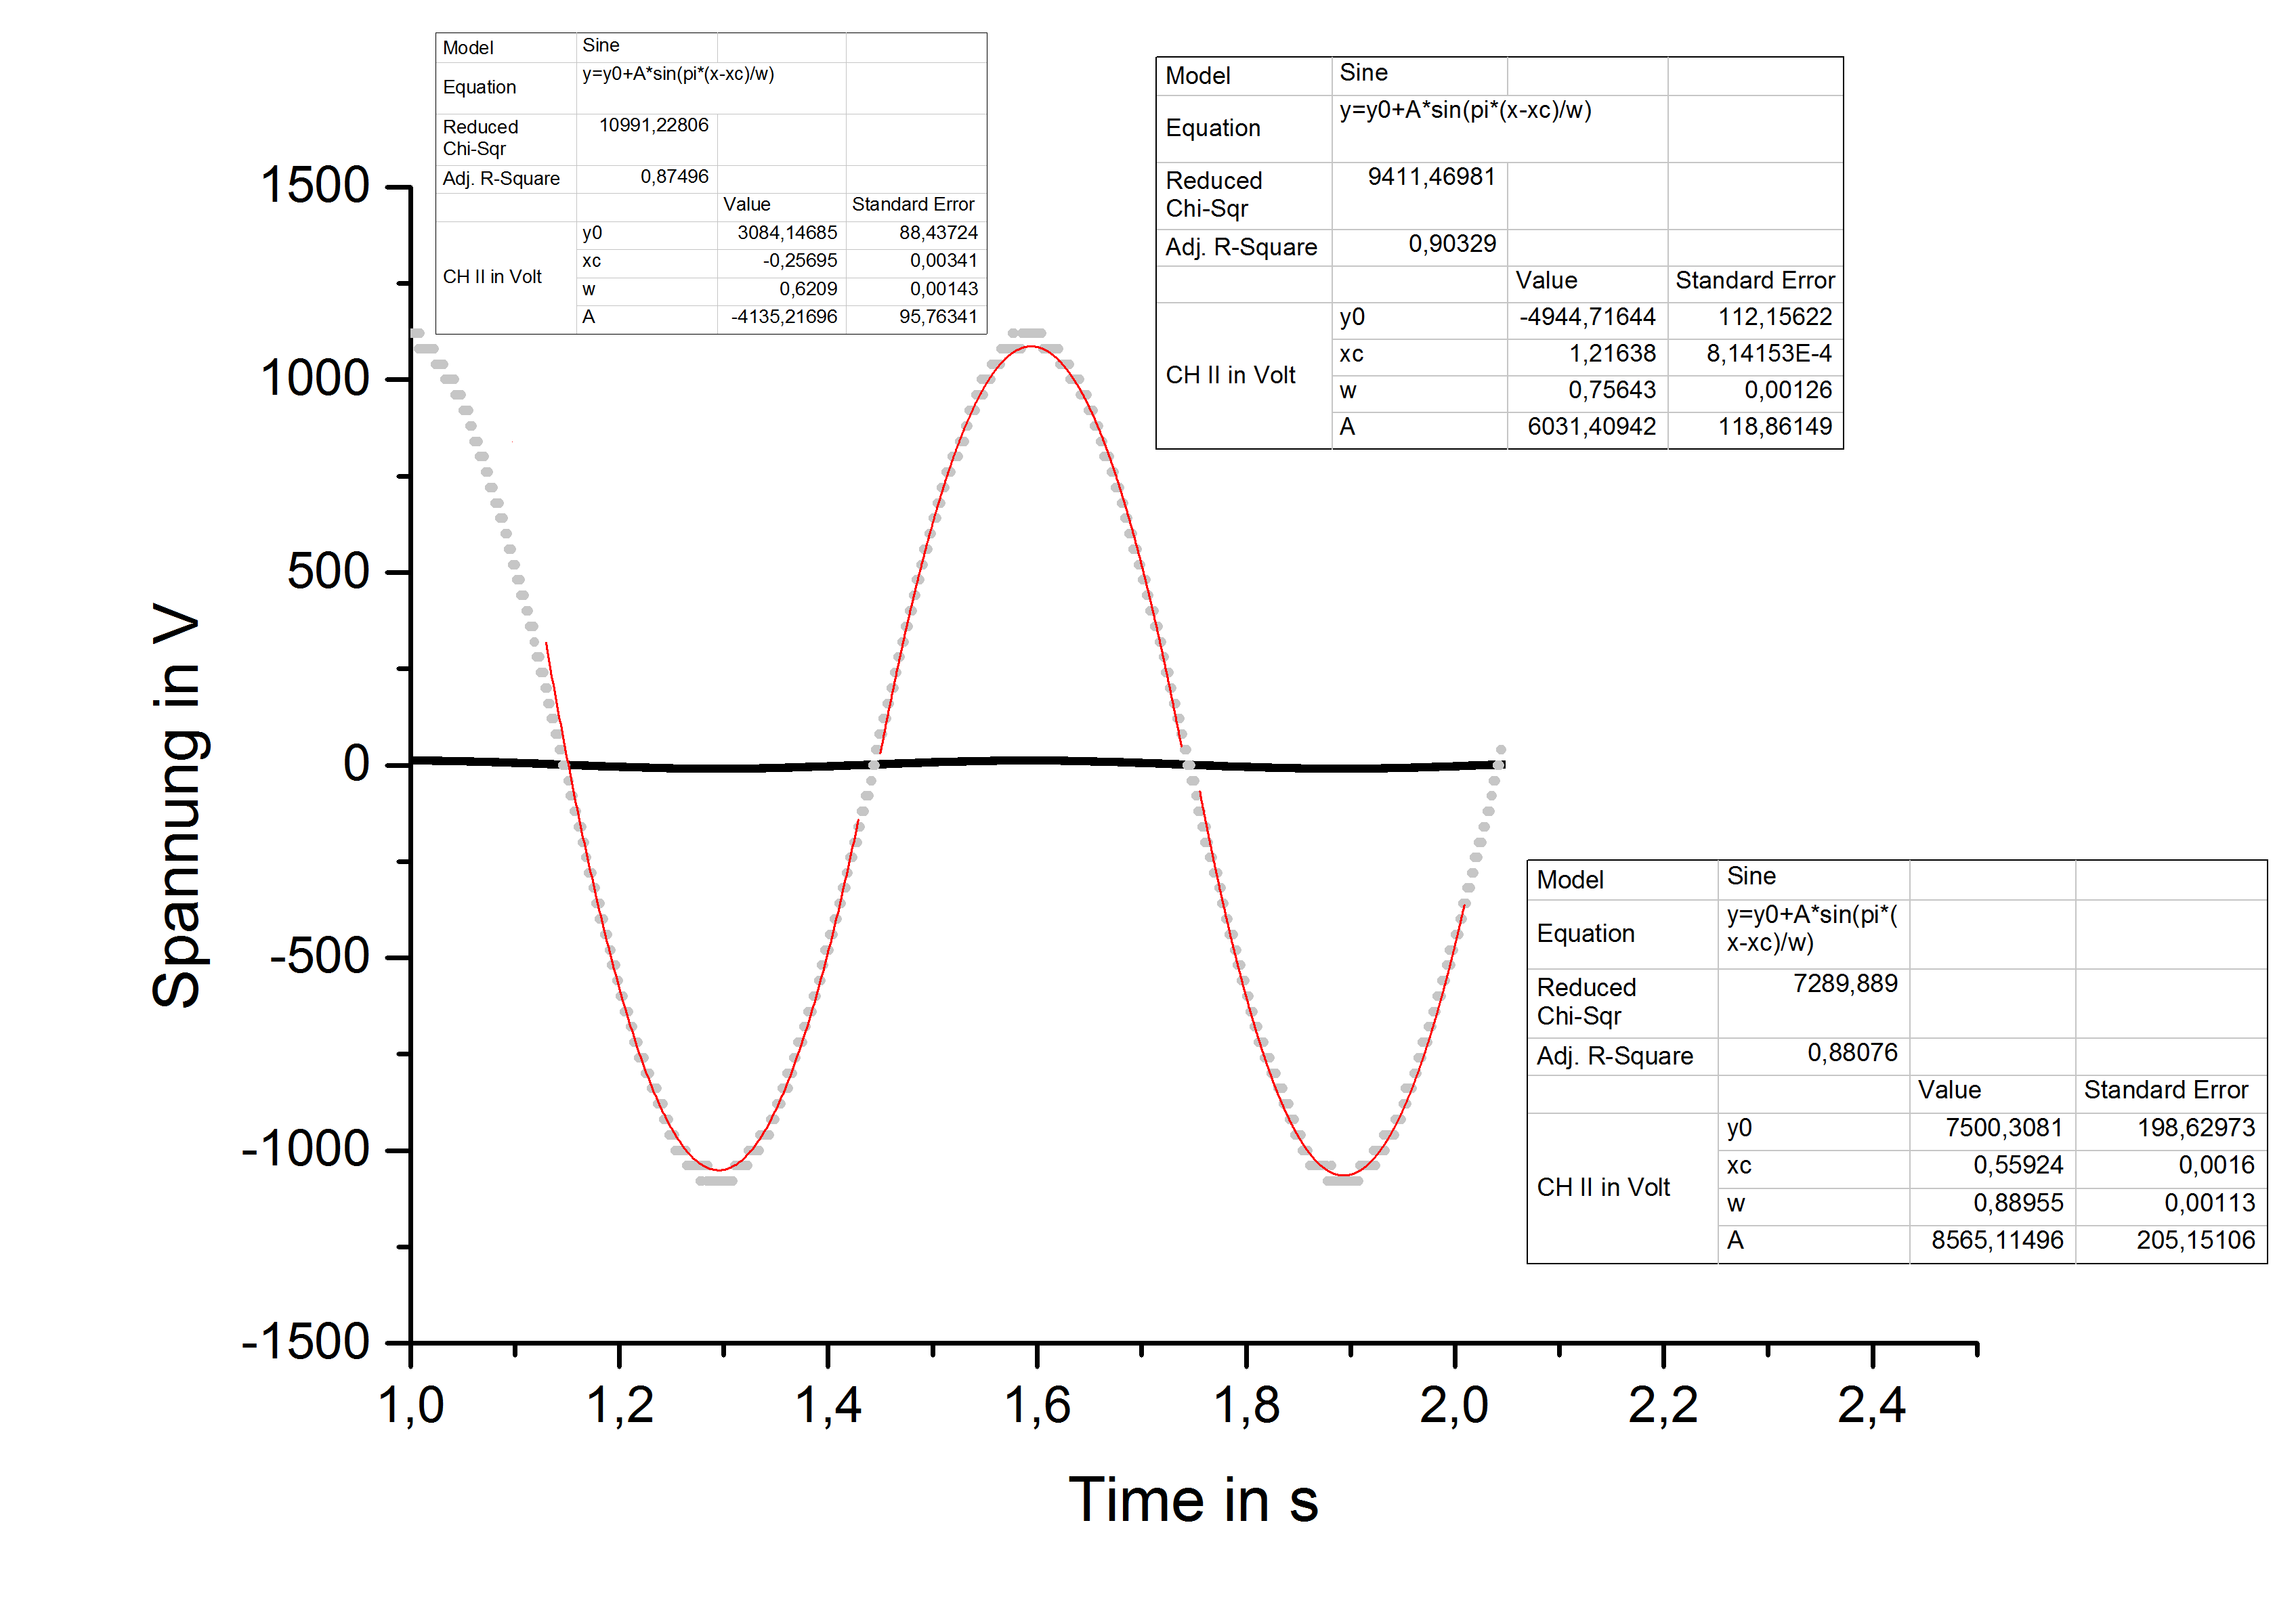
\includegraphics[scale=0.5]{verstaerkt.png}
\caption{Signal ohne Drosselung}
\end{center}
\end{figure}
\clearpage
\begin{figure}[h]
\begin{center}
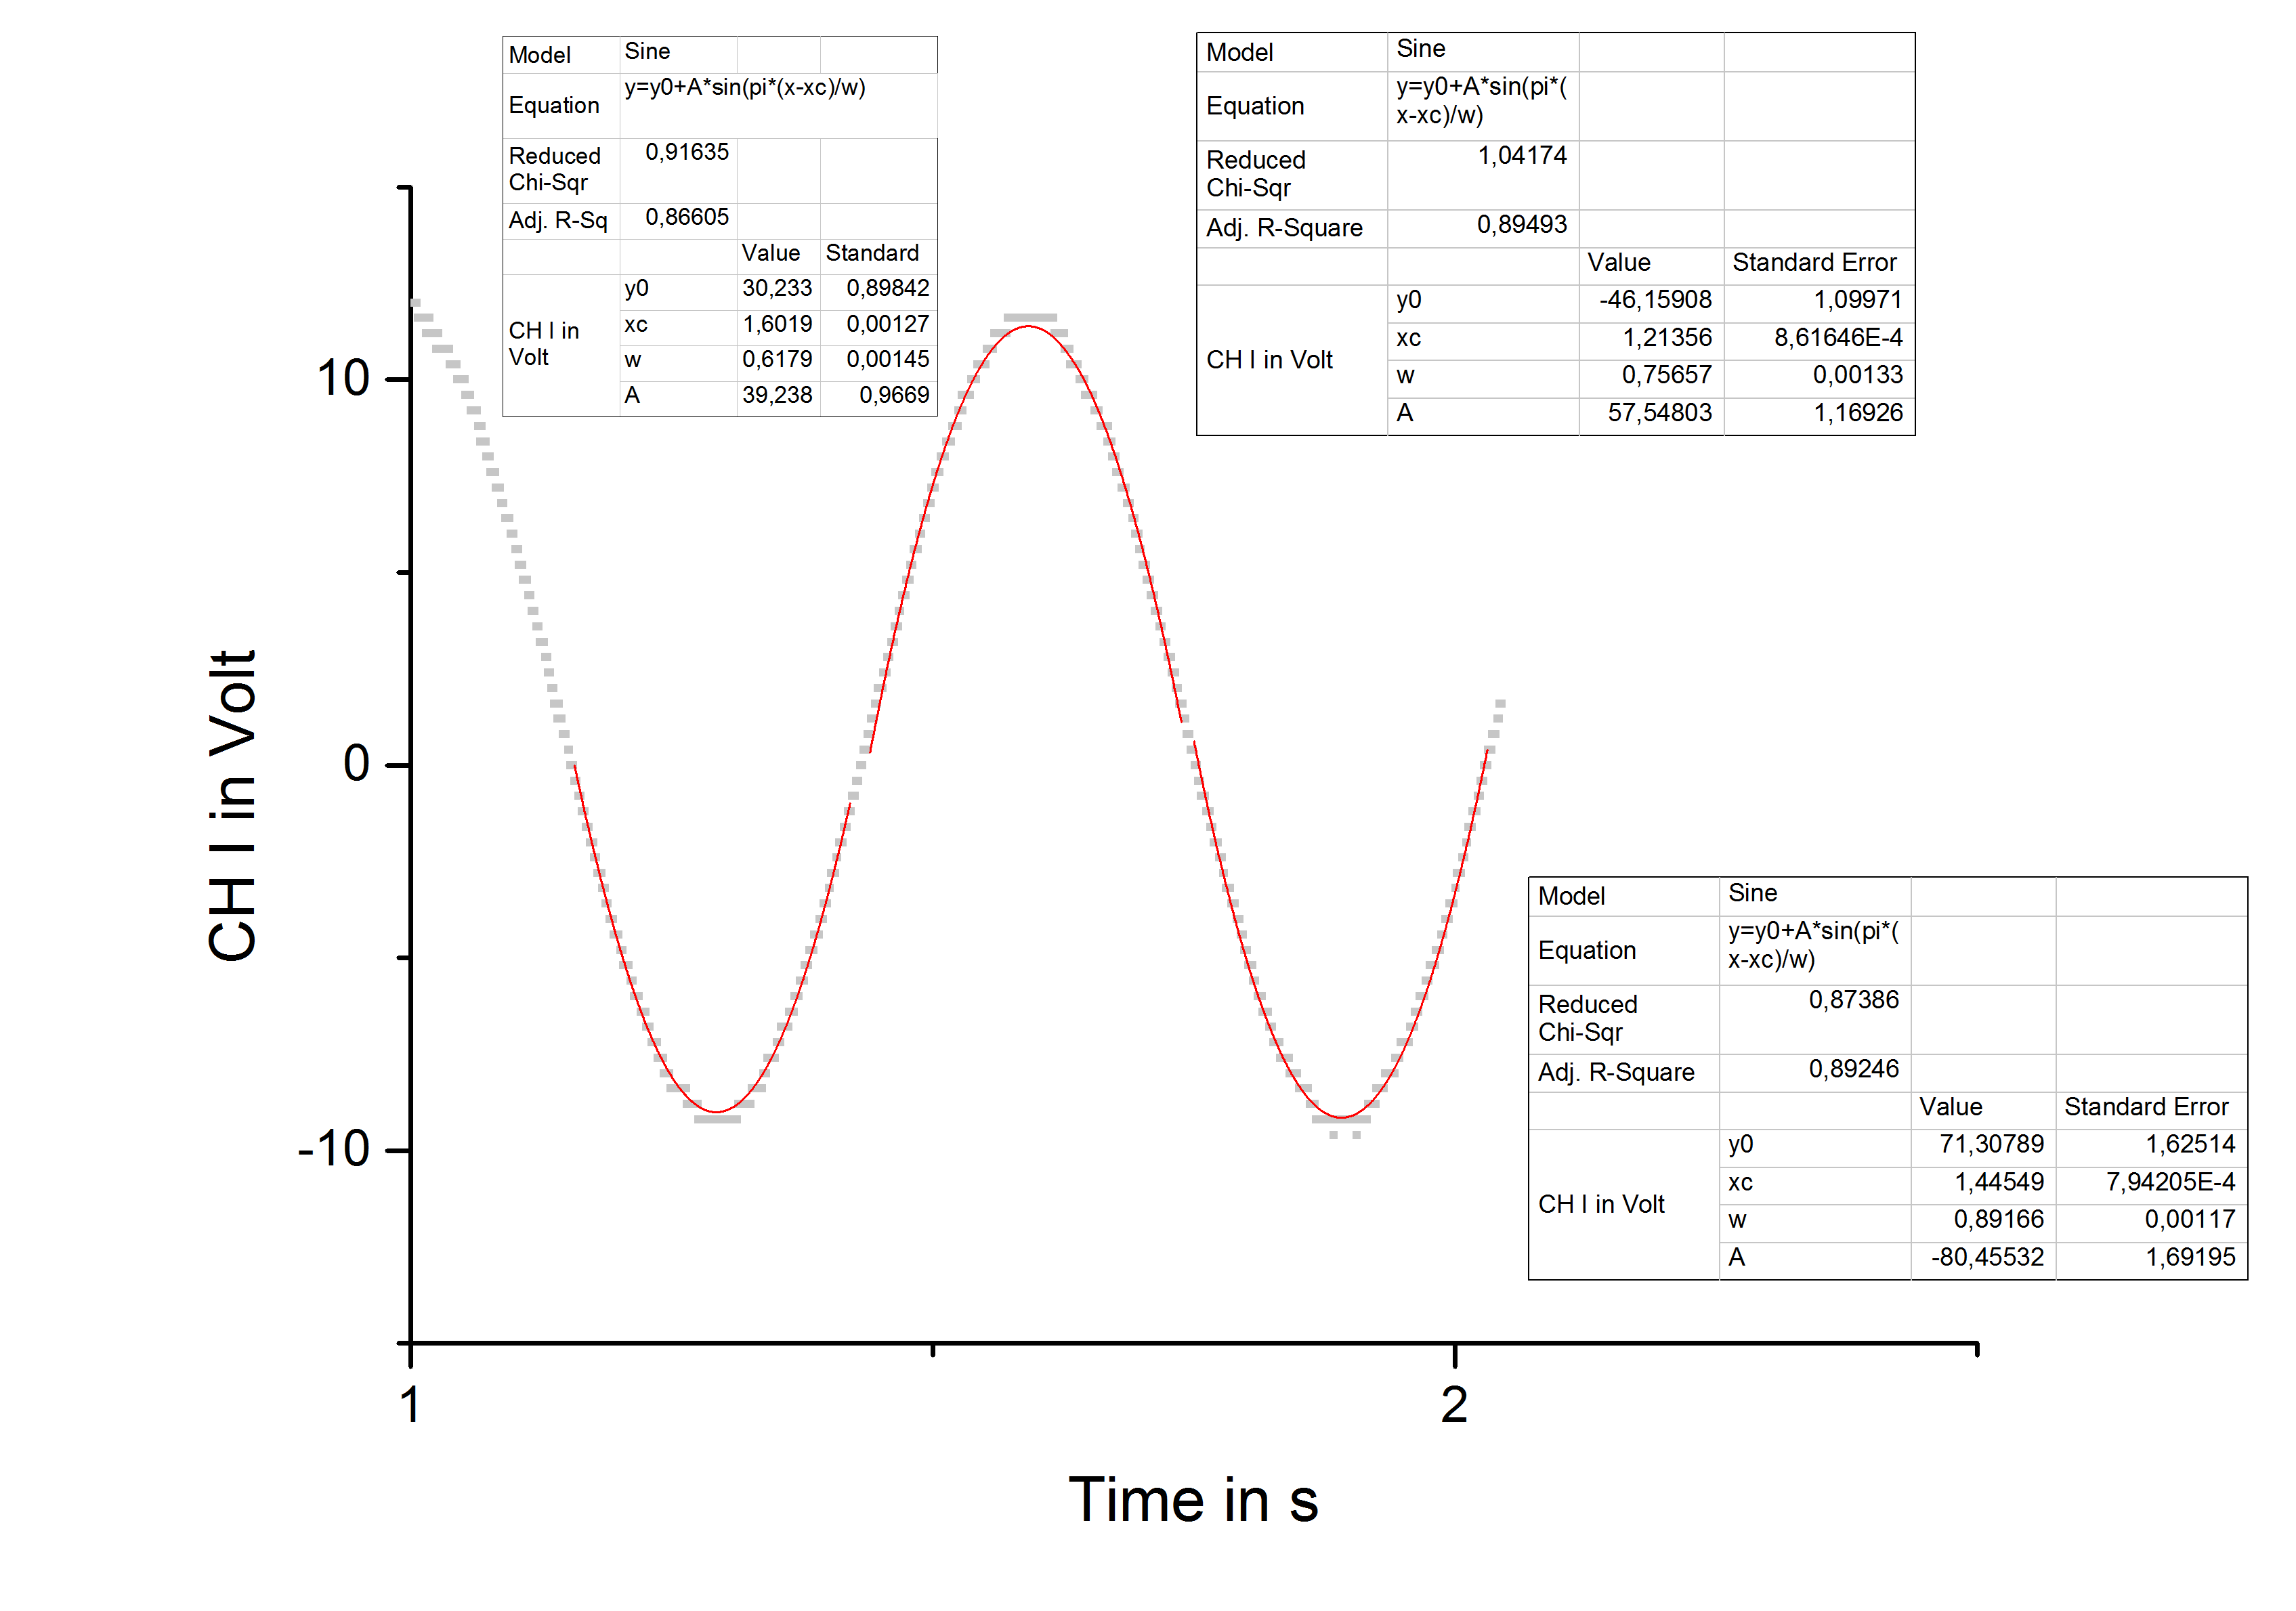
\includegraphics[scale=0.5]{ch1t23.png}
\caption{Gedrosseltes Signal}
\end{center}
\end{figure}
Die tatsächliche Amplitude errechneten wir mit den Formeln $A+y_{0}$ bzw. $y_{0}-A$, je nachdem, wie Origin den Fit erstellte. Für den Fehler gilt: \\
$\Rightarrow s_{Ampl.}=\sqrt{s_{A}^{2}+s_{y_{0}}^{2}}$\\
Für den Faktor, mit welchem die Werte tatsächlich hätten multipliziert werden müssen, gilt somit:\\
\[D=\frac{Ampl_{normal}}{Ampl_{gedrosselt}}\]
\[\Rightarrow s_D=D*\sqrt{(\frac{s_{Ampl_{normal}}}{Ampl_{normal}})^{2}+(\frac{s_{Ampl_{gedrosselt}}}{Ampl_{gedrosselt}})^{2}}\]
Insgesamt erhielten wir 9 Peaks, welche allesamt nach derselben Methode ausgewertet wurden. Für die Verhältnisse der Amplituden gilt:\\
\begin{table}[htbp]
\begin{tabular}{|r|r|r|}
\hline
\multicolumn{1}{|l|}{Peaks} & \multicolumn{1}{l|}{D\_i} & \multicolumn{1}{l|}{s\_D\_i} \\ \hline
1 & 91,4 & 19,6 \\ \hline
2 & 123,8 & 24,0 \\ \hline
3 & 124,6 & 52,1 \\ \hline
4 & 93,3 & 20,6 \\ \hline
5 & 120,7 & 42,7 \\ \hline
6 & 124,1 & 20,5 \\ \hline
7 & 95,4 & 19,7 \\ \hline
8 & 116,4 & 43,2 \\ \hline
9 & 116,7 & 22,4 \\ \hline
\end{tabular}
\end{table}
\clearpage
Da hierbei nur Verhältnisse berechnet wurden, haben wir die Fehler des Oszilloskops vernachlässigt.\\
Um schließlich $\bar{D}$ zu berechnen, verwendeten wir eine gewichtete Mittelung:\\
\[\bar{D}=\sum\limits_{i=1}^{9}\frac{\frac{D_{i}}{\sigma_{i}^{2}}}{\frac{1}{\sigma_{i}^{2}}}\]
Für den Fehler gilt: \\
\[s_{\bar{D}}=\sum\limits_{i=1}^{9}\frac{1}{\frac{1}{\sigma_{i}^{2}}}\]
Somit erhielten wir: \\
$\bar{D}=(107\pm8)$\\
Im Rahmen der Standardabweichung handelt es sich also tatsächlich um eine Verstärkung um den Faktor 100. Um einen genaueren Wert zu erhalten, rechneten wir allerdings:\\
\[U_{\lambda/2}=\frac{\bar{D}}{100}*U\]
Für den Fehler folgt dann mit Gauss'scher Fehlerfortpflanzung:\\
\[s_{U_{\lambda/2}}=\sqrt{(\frac{U_{\lambda/2}}{100})^{2}*s_{\bar{D}}^{2}+(\frac{\bar{D}}{100})^{2}*s_{U_{\lambda/2}}^{2}}\]
Somit erhielten wir:\\
$U_{\lambda/2}=(240\pm30)V$\\
Den elektrooptischen Koeffizienten $r_{41}$ errechneten wir mit der in [Ver] gegebenen Formel (und den dort gegebenen Konstanten):\\
\[r_{41}=\frac{\lambda*d}{4l*U_{\lambda/2}}*\left(\sqrt{0,5*(\frac{1}{n_{1}^{2}}+\frac{1}{n_{3}^{2}})}\right)^{3}=23,4 \frac{pm}{V}\]
Für den Fehler gilt:\\
\[s_{r_{41}}=r_{41}*\frac{s_{U_{\lambda/2}}}{U_{\lambda/2}}=2,8 \frac{pm}{V}\]
Insgesamt gilt also:\\
$r_{41}=(23\pm3)\frac{pm}{V}$\\
Der Literaturwert beträgt $23,4\frac{pm}{V}$. Der mithilfe unserer Messwerte errechnete Wert liegt im Rahmen einer Standardabweichung auf dem Literaturwert. 
\subsubsection{Sinusmodulierte Gleichspannungsmethode}
Bei dieser Messreihe wurde an die von einer Gleichspannung überlagerte Sinusspannung an die Pockelszelle angelegt. Wir veränderten den Gleichspannungsanteil, bis eine Verdopplung der Frequenz am Oszilloskop sichtbar war. Diese Spannung notierten wir. Wir taten dies für negative wie für positive Spannungen jeweils 10-mal (für die Messreihe s. Anhang). Somit errechneten wir $U_{\lambda/2}$ folgendermaßen:\\
\[\overline{U_{pos}}=\frac{1}{10}\sum\limits_{i=1}^{10}U_{pos_{i}}\]
Der Fehler errechnete sich als reiner statistischer Fehler, da uns für das Gerät kein Fehler der Anzeige bekannt war, weshalb wir diesen vernachlässigten (wodurch die Fehler zu klein sind):\\
\[s_{\overline{U_{pos}}}=\sqrt{\frac{1}{9}\cdot\sum\limits_{i=1}^{10}\left(U_{pos_{i}}-\overline{U_{pos}}\right)^{2}}\]
Für die negativen Spannungen wurden die Werte analog berechnet. Somit erhielten wir:\\
$\overline{U_{pos}}=(129,4\pm0,2)V$\\
$\overline{U_{neg}}=(-121,8\pm0,4)V$\\
Für $U_{\lambda/2}$ gilt somit:\\
\[U_{\lambda/2}=\overline{U_{pos}}-\overline{U_{neg}}=251,2 V\] und für den Fehler: \[s_{U_{\lambda/2}}=\sqrt{s_{\overline{U_{pos}}}^{2}+s_{\overline{U_{neg}}}^{2}}=0,5 V\]
Analog zum vorherigen Kapitel errechneten wir damit den elektrooptischen Koeffizienten und erhielten:\\
$r_{41}=(22,41\pm0,04)\frac{pm}{V}$
Der Fehler ist, wie bereits erwähnt, zu klein. Dennoch ist auch zu beobachten, dass der Wert selbst nicht so genau ist wie der mithilfe der Sägezahnmethode bestimmte. Dies könnte auf einen systematischen Fehler hinweisen, beispielsweise durch eine nicht vorgesehene Erwärmung der Kristalle, was die natürliche Doppelbrechung beeinflussen kann.


